\begin{frame}{Sensores basados en la tecnología CMOS}
	\centering
	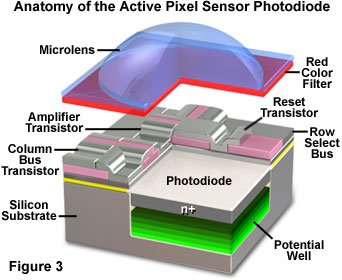
\includegraphics[height=.65\textheight]{aps.jpg}
\end{frame}%

\begin{frame}{Nuevos sensores basados en la tecnología CMOS}
	\centering
	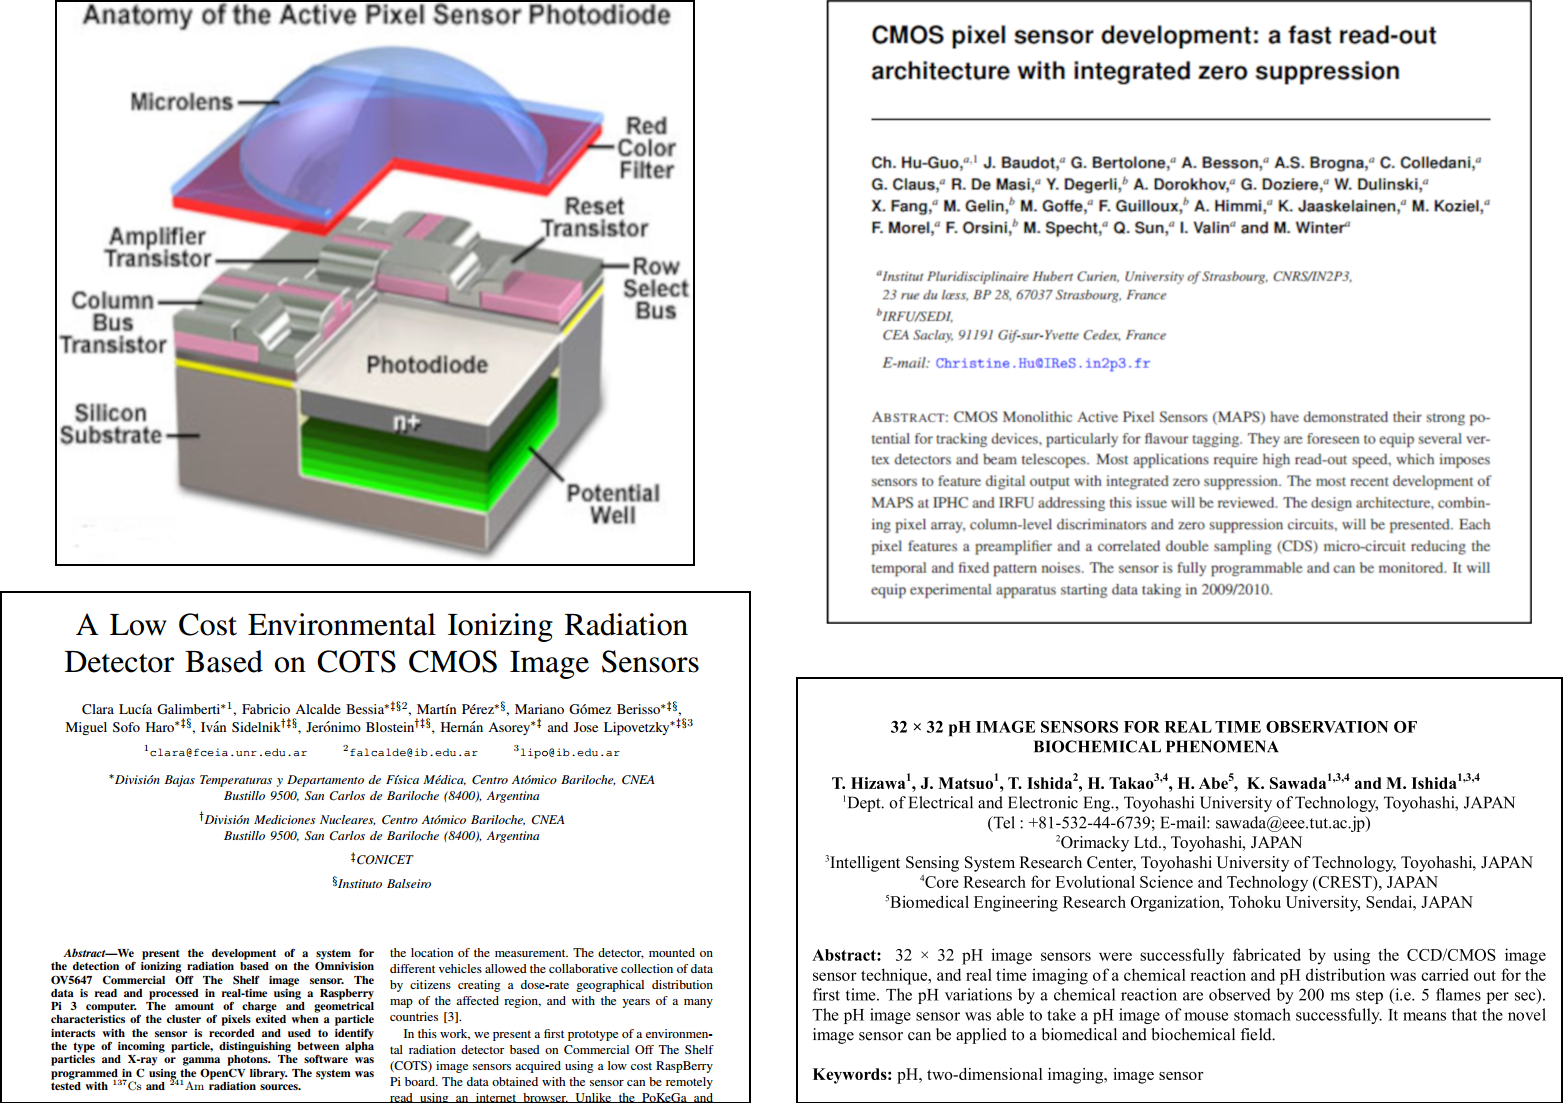
\includegraphics[height=.8\textheight]{sensores3.png}
\end{frame}

\begin{frame}{Nuevos sensores basados en la tecnología CMOS}
	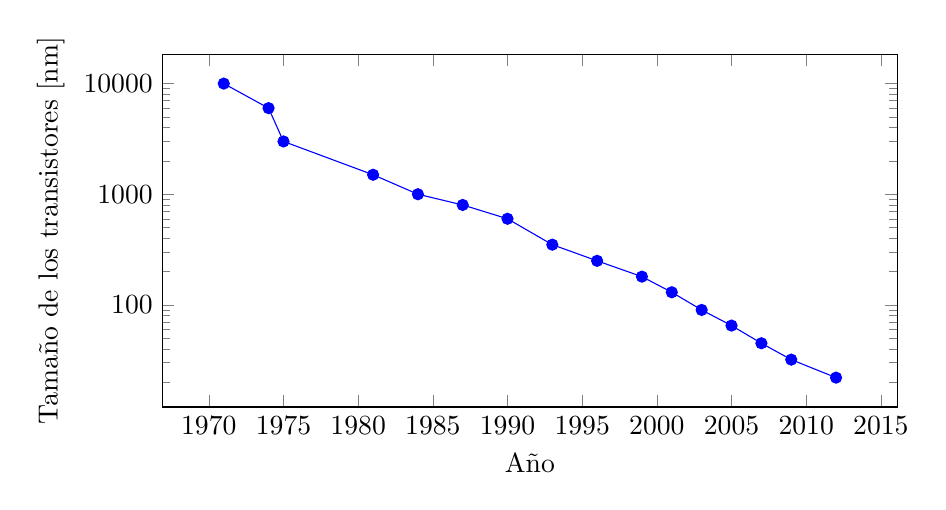
\begin{tikzpicture}
	\begin{semilogyaxis}[
	height=0.5\textwidth,
	width=.9\textwidth,
	xlabel=Año,
	xtick={1970,1975,...,2025},
	ylabel={Tamaño de los transistores [nm]},
	ymode=log,
	log ticks with fixed point,
	tick label style={/pgf/number format/1000 sep={}}
	]
	\addplot[mark=*,blue] coordinates {(1971,10000)(1974,6000) (1975,3000) (1981,1500)(1984,1000)(1987,800)(1990,600)(1993,350)(1996,250)(1999,180)(2001,130)(2003,90)(2005,65)(2007,45)(2009,32)(2012,22)};
	\end{semilogyaxis}
	\end{tikzpicture}
	\blfootnote{https://en.wikipedia.org/wiki/Moore's\_law}
\end{frame}

\begin{frame}[c]{Comunicación USB 2.0 para sistema científicos implementados en FPGA}
	\centering
%	\only<1>{
		\begin{tikzpicture}[>=latex]
			\node[bloque](pc){PC};
			\node[bloque](adq)[right =1.3 of pc]{Sistema de adquisicíon basado en FPGA};
			\node[bloque](sens)[right=1.3 of adq]{Sensor para datos científicos};
			\draw[<->,double]([yshift=10]pc.east) -- node [above]{Datos} ([yshift=10]adq.west);
			\draw[<->,double]([yshift=-10]pc.east) -- node [above]{Control} ([yshift=-10]adq.west);				
			\draw[<->,double]([yshift=10]adq.east) -- node [above]{Datos} ([yshift=10]sens.west);
			\draw[<->,double]([yshift=-10]adq.east) -- node [above]{Control} ([yshift=-10]sens.west);
		\end{tikzpicture}
%	}
%	\only<3>{
%		\begin{tikzpicture}[>=latex,scale=1.5]
%			\begin{scope}[transform shape]
%				\node[bloque](pc){PC};
%				\node[bloque](adq)[right =3 of pc]{Sistema de adquisicíon basado en FPGA};
%				\draw[<->,ultra thick]([yshift=5]pc.east) -- node (data)[above]{Datos} ([yshift=5]adq.west);
%				\draw[<->,ultra thick]([yshift=-20]pc.east) -- node (ctrl)[above]{Control} ([yshift=-20]adq.west);
%			\end{scope}
%			\begin{scope}[on background layer]
%				\node[rounded rectangle,fill=red!30,fit=(pc.east)(adq.west)(data)(ctrl)]{};
%			\end{scope}				
%		\end{tikzpicture}}
%	\only<2>{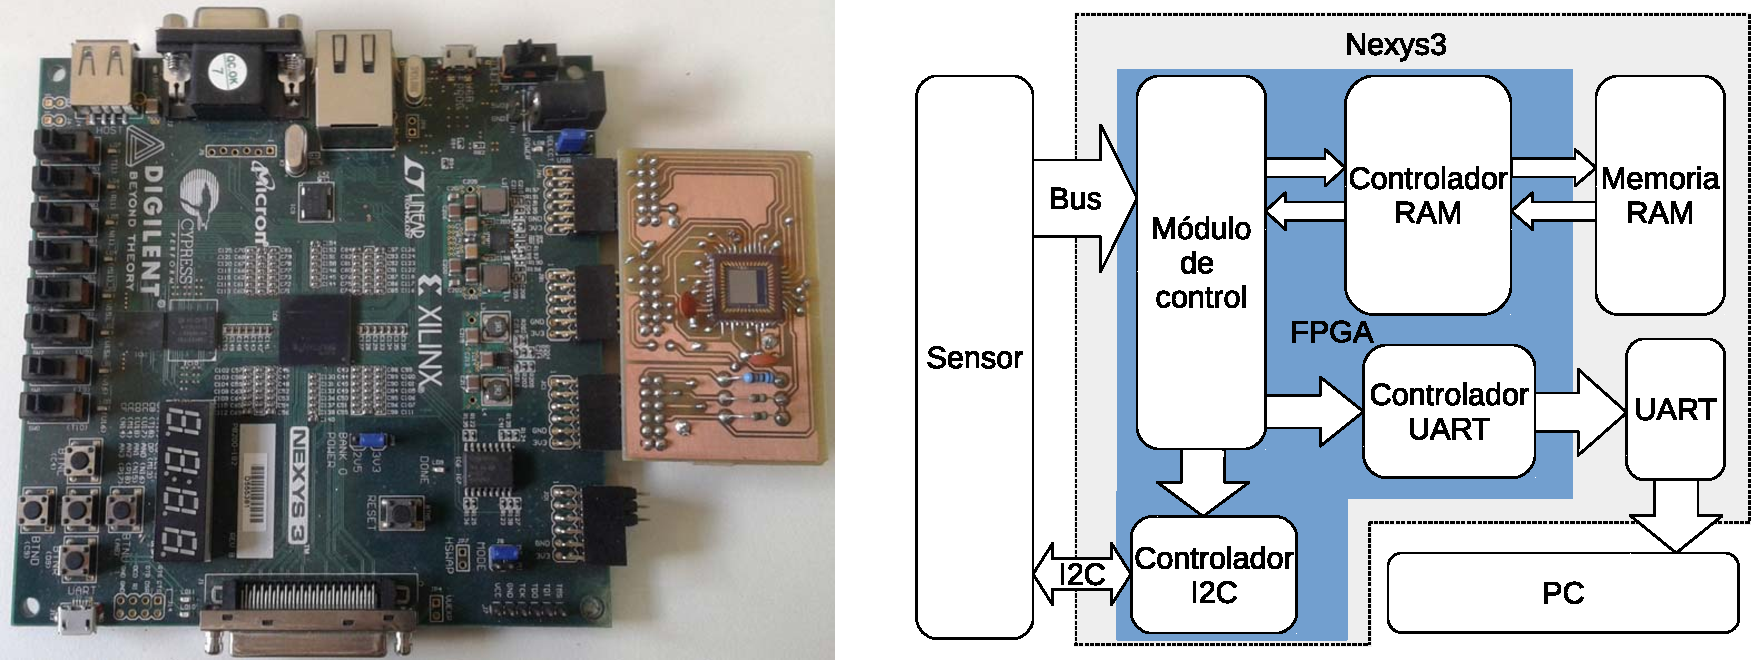
\includegraphics[width=0.9\paperwidth]{01motivacion}}
\end{frame}
%
%
%\begin{frame}{La producción de información científica}
%	\framesubtitle{¿Por qué es los científicos necesitan nuevos sensores?}
%	\centering	
%	\begin{tikzpicture}
%		\node(gerschman) {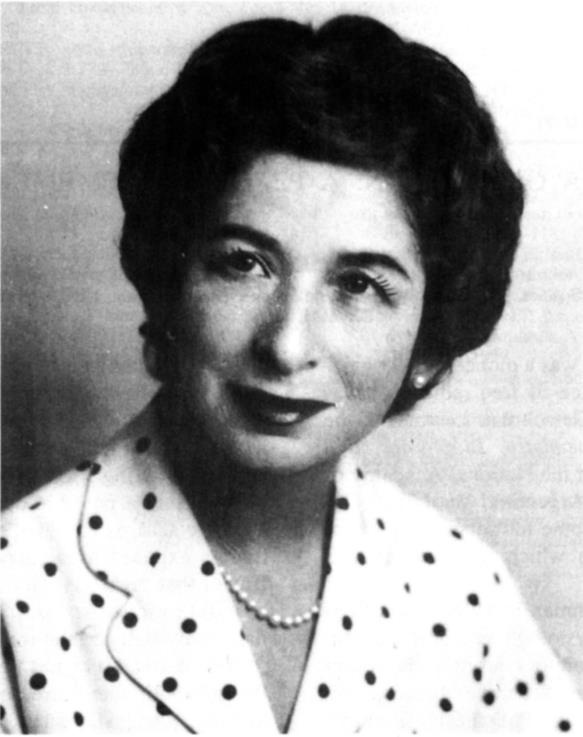
\includegraphics[width=.15\textwidth]{gerschman.jpg}};
%		\node[visible on=<2->](auger)[right=of gerschman]{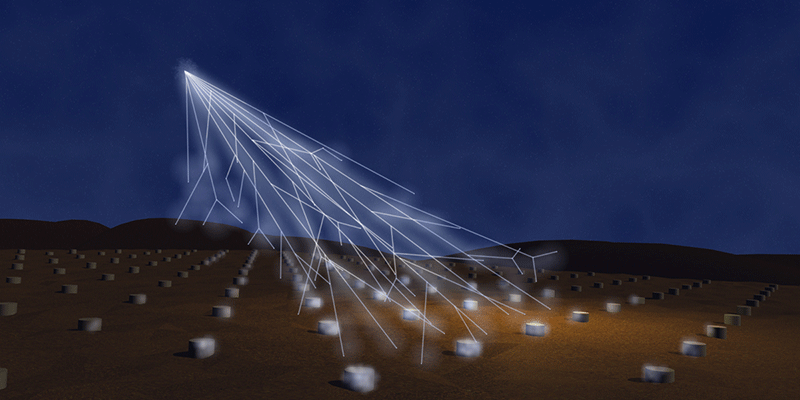
\includegraphics[width=.25\textwidth]{pierreauger.png}};
%		\draw[visible on=<2->,lineaExt](gerschman)--(auger);
%		\draw[visible on=<2->,lineaInt](gerschman)--(auger);
%		\node[visible on=<3->](medipix)[right=of auger]{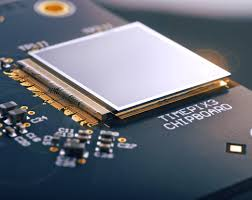
\includegraphics[width=.2\textwidth]{medipix.jpg}};
%		\draw[visible on=<3->,lineaExt](auger)--(medipix);
%		\draw[visible on=<3->,lineaInt](auger)--(medipix);
%	\end{tikzpicture}
%\only<1->{\blfootnote{https://mujeresconciencia.com}}
%\only<2->{\blfootnote{https://physics.aps.org}}
%\only<3->{\blfootnote{https://medipix.web.cern.ch}}
%
%\end{frame}
%
%\begin{frame}{Nuevos sensores basados en la tecnología CMOS}
%	\centering
%	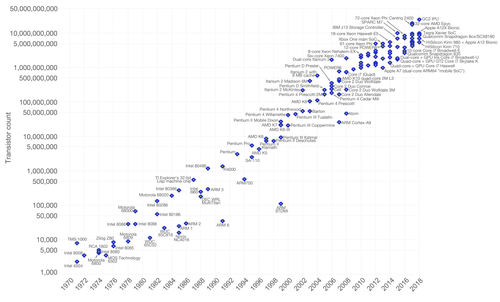
\includegraphics[width=\textwidth]{leyDeMoore.png}
%	\blfootnote{https://en.wikipedia.org/wiki/Moore's\_law}
%\end{frame}
%	

%

%

%
%\begin{frame}{Adquisidores de datos con alta velocidad}
%	\centering
%	\begin{columns}[]
%		\begin{column}{.40\textwidth}
%			\centering
%			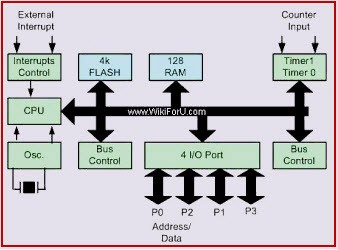
\includegraphics[height=.3\textheight]{uc.jpg}
%			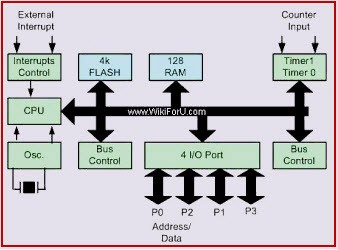
\includegraphics[width=.8\columnwidth]{uc.jpg}
%		\end{column}
%		\begin{column}{.40\textwidth}
%			\centering
%			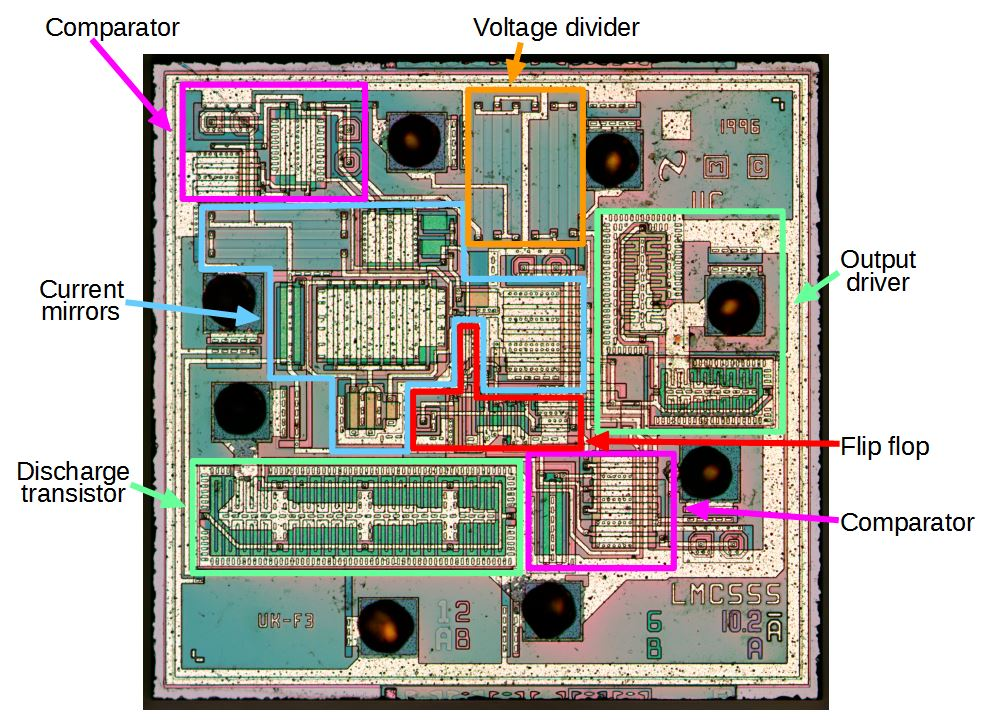
\includegraphics[width=.9\columnwidth]{asic2.jpg}
%		\end{column}
%	\end{columns}
%	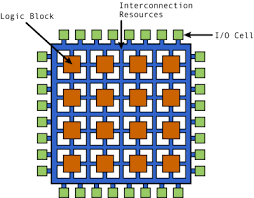
\includegraphics[width=.45\textwidth]{fpga.png}
%\end{frame}
%
%\begin{frame}{FPGA como adquisidor y procesador de datos}
%	\centering
%	\begin{columns}
%		\begin{column}{.4\textwidth}
%			\centering
%			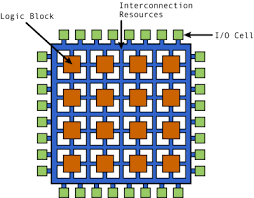
\includegraphics[width=\textwidth]{fpga.png}
%		\end{column}
%		\begin{column}{.4\textwidth}
%			\centering
%			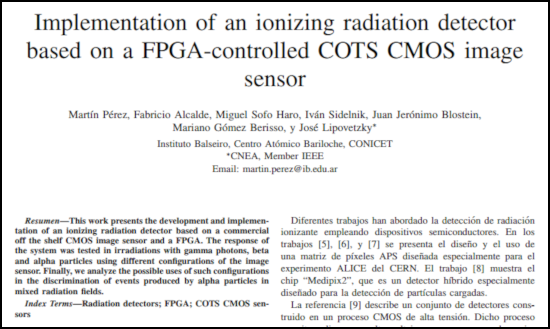
\includegraphics[width=\textwidth]{fpgapapers.png}
%		\end{column}
%	\end{columns}
%\end{frame}
%
%\begin{frame}{La PC como procesador de datos}
%	\centering
%	\begin{tikzpicture}[node distance=.2]
%		\node (pc) {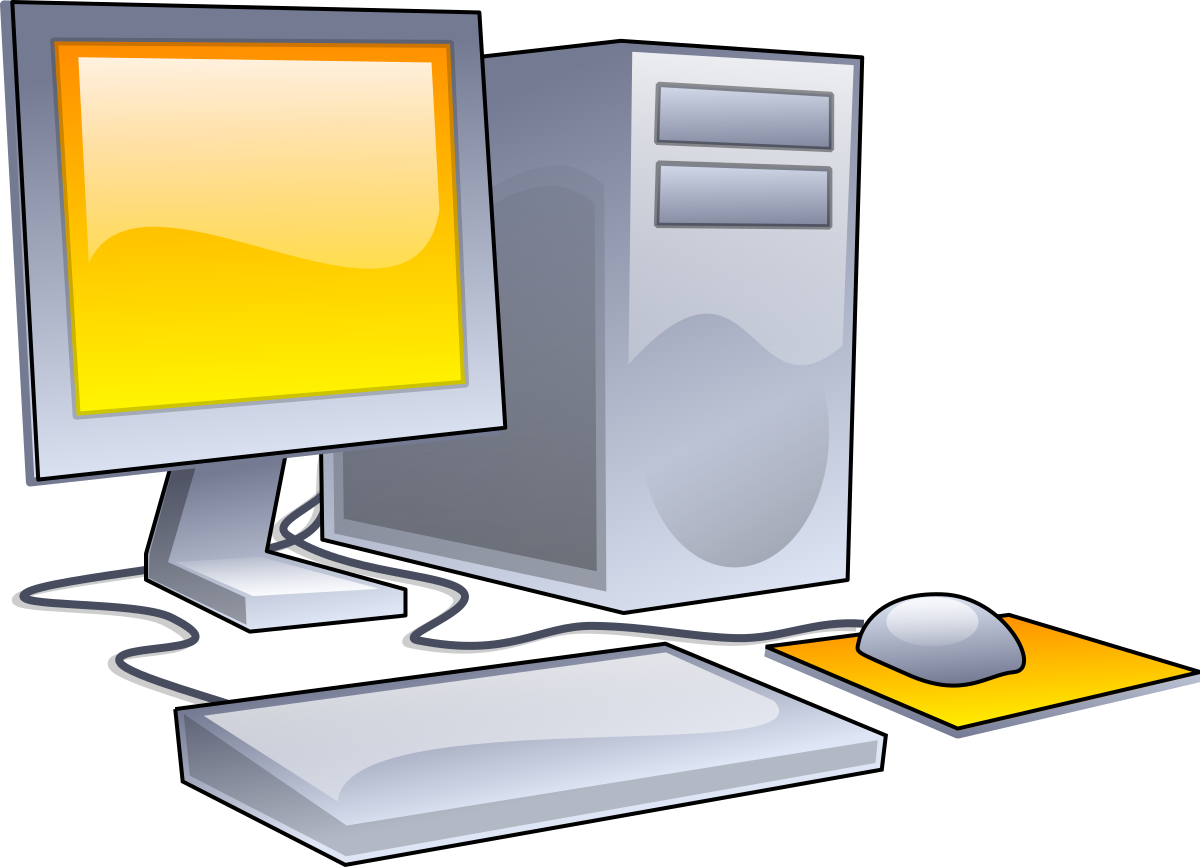
\includegraphics[width=.35\textwidth]{pc}};
%		\node[visible on=<2->] (matlab) [above left=of pc] {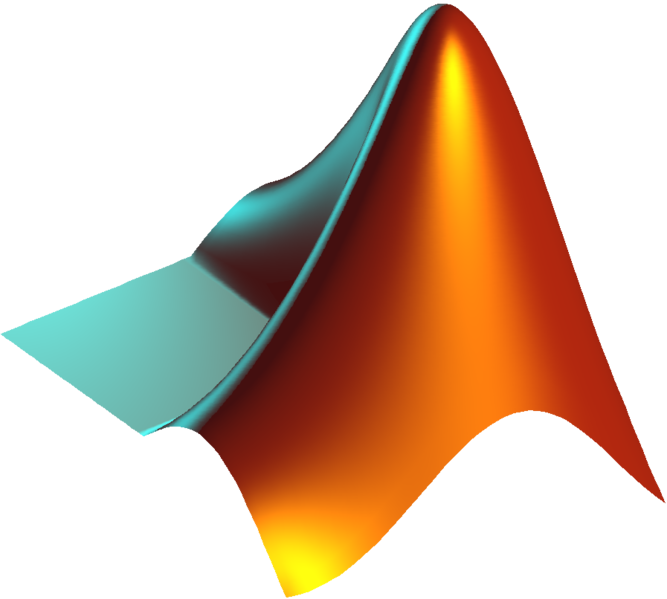
\includegraphics[width=.15\textwidth]{matlab.png}};
%		\node[visible on=<2->] (python) [below right=of pc] {
\includegraphics[width=.15\textwidth]{python}};
%		\node[visible on=<3->] (ros) [below left=of pc]{
\includegraphics[width=.15\textwidth]{ros}};
%		\node[visible on=<4->] (origin)[above right=of pc]{
\includegraphics[width=.15\textwidth]{origin}};
%		\node[visible on=<5->] (cloud) [above=of pc]{
\includegraphics[width=.15\textwidth]{cloud.jpg}};
%	\end{tikzpicture}
%\end{frame}
%
%\begin{frame}{La necesidad de una comunicación\\entre un FPGA y una PC}
%		\centering
%		\begin{tikzpicture}[>=latex,scale=1.5]
%			\begin{scope}[transform shape]
%				\node[bloque](pc){PC};
%				\node[bloque](adq)[right =3 of pc]{Sistema de adquisicíon basado en FPGA};
%				\draw[<->,ultra thick]([yshift=5]pc.east) -- node (data)[above]{Datos} ([yshift=5]adq.west);
%				\draw[<->,ultra thick]([yshift=-20]pc.east) -- node (ctrl)[above]{Control} ([yshift=-20]adq.west);
%			\end{scope}
%			\begin{scope}[on background layer]
%				\node[rounded rectangle,fill=red!30,fit=(pc.east)(adq.west)(data)(ctrl)]{};
%			\end{scope}				
%		\end{tikzpicture}
%\end{frame}
%
\begin{frame}{Selección del protocolo de comunicación}
%	\begin{itemize}
		\begin{columns}
			\begin{column}{.28\textwidth}
				\centering 
				Ethernet\\
%				\item Ethernet\\
				\vspace{1mm}
				\centering 
				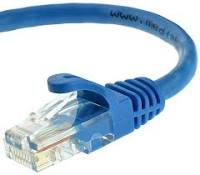
\includegraphics[height=.18\textheight]{ethernet}
			\end{column}
			\begin{column}{.28\textwidth}
				\centering
				Wi-Fi\\
%				\item Wi-Fi\\
				\vspace{1mm}
				\centering 
				
\includegraphics[height=.18\textheight]{wifi}
			\end{column}
			\begin{column}{.28\textwidth}
				\centering
%				\item USB\\
				USB\\
				\vspace{1mm}
				\centering
				
\includegraphics[height=.18\textheight]{usb20}
			\end{column}
		\end{columns}
%	\end{itemize}
	\vspace{2cm}
	\only<2>{\centering \large{USB 2.0 resulta la mejor alternativa para comunicar periféricos a una PC sin comprometer funcionalidades importantes.\\}}
\end{frame}